\chapter{Feature importances} % Main appendix title
\label{app:feature_importances}

\section{F1 feature importances}
\subsection{FAHES \& ForbiddenItemSets}
Due to the low average F1-scores for FAHES \& ForbiddenItemSets, it is not possible to extract any SHAP values from the estimators, as the estimate for the F1 is equal to 0. Whilst it was possible to extract interpretations from the precision and recall estimators, these will not be discussed as this is out of scope for this research for now.

\subsection{ActiveClean}
For ActiveClean, the 10 most influential features are shown in figure \ref{fig:most_impact_features_activeclean}. The estimators base the F1 prediction mainly on the variance of characteristics across the different columns a dataset has. Meaning that, if the characteristics of columns differ from each other, the variance for that feature will be higher.

\begin{figure}[H]
    \centering
    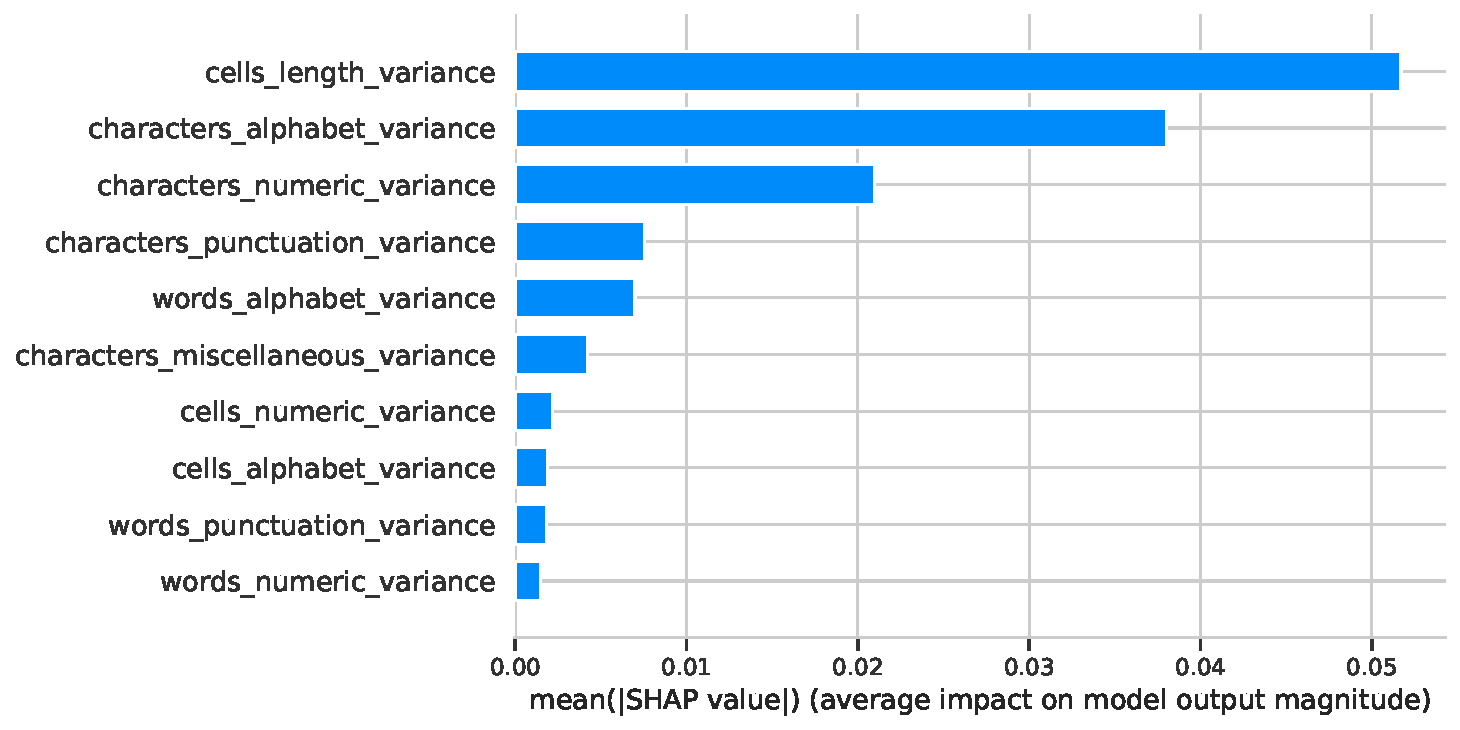
\includegraphics[width=0.9\textwidth]{thesis/Figures/RQ4/Shap_cell_f1_ActiveClean.pdf}
    \caption{ActiveClean - Top 10 influential features according to SHAP values}
    \label{fig:most_impact_features_activeclean}
\end{figure}

The top 3 features and their correlation with impact are displayed in table \ref{tab:top_influence_features_activeclean}. When the cells\_length\_variance is higher, the performance result will be estimated lower. This means that if different columns, have different content sizes, the error detection job most likely becomes harder. This happens with heterogeneous relational data with many different data types and lengths. Also, when there is a lot of difference between the use of alphabetical characters between columns (characters\_alphabet\_variance), so some have many alphabetical characters, others do not, the performance decreases. Lastly, whenever the characters\_numeric\_variance is higher, the performance will increase. This means that if there are columns that have many numerical characters and other columns are non-numerical, it is easier for ActiveClean to differentiate errors. These results can be the effect of the featurizer, tf–idf (term frequency–inverse document frequency), which relies on the frequency of words and word pairs occuring in that data. So if the lengths of attributes and the number of alphabetical characters per column are generally the same, but there are some columns numerical, it is able to correctly group these rows and do error detection.

\begin{table}[H]
\centering
\begin{tabular}{llr}
\toprule
 \# &                         Feature &         Influence \\
\midrule
 1 &         cells\_length\_variance &  -0.48 $\searrow$ \\
 2 &  characters\_alphabet\_variance &  -0.56 $\searrow$ \\
 3 &   characters\_numeric\_variance &   0.42 $\nearrow$ \\
\bottomrule
\end{tabular}
\caption{ActiveClean - Top 3 feature influence}
\label{tab:top_influence_features_activeclean}
\end{table}


\subsection{dBoost}
For dBoost, the 10 most influential features are shown in figure \ref{fig:most_impact_features_dboost}. 

\begin{figure}[H]
    \centering
    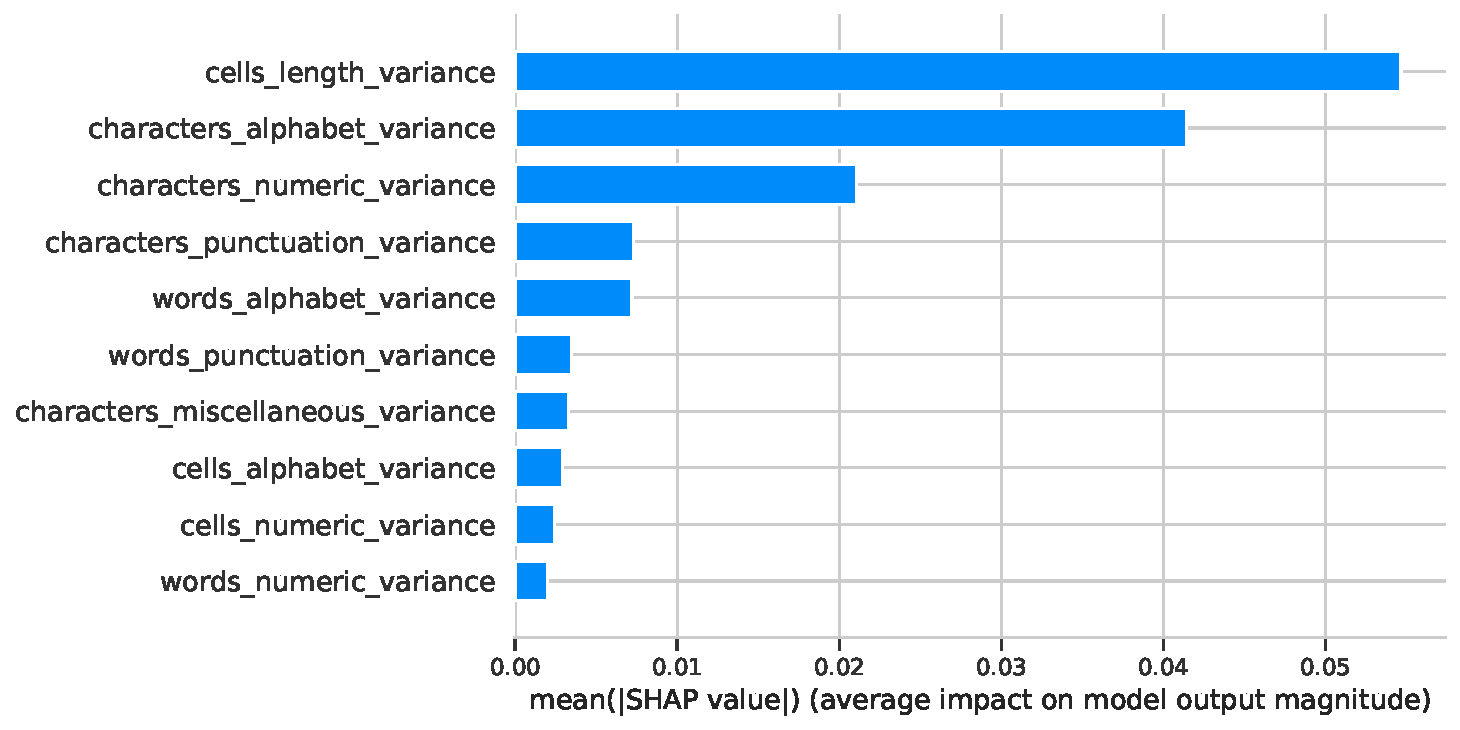
\includegraphics[width=0.9\textwidth]{thesis/Figures/RQ4/Shap_cell_f1_dBoost.pdf}
    \caption{dBoost - Top 10 influential features according to SHAP values}
    \label{fig:most_impact_features_dboost}
\end{figure}

The top 3 impactful features for dBoost are the same as for ActiveClean. However, the influence of the features is different \ref{tab:top_influence_features_dboost}. if the length of cells across varies more, the performance of dBoost decreases more drastically. The variance in numerical characters does have a high impact on the performance, but no direct correlation, meaning that depending on different features, it might have a positive or negative impact. 
Concluding, dBoost will perform best in structured data with the same length of cells across the columns.

\begin{table}[H]
\centering
\begin{tabular}{llr}
\toprule
 \# &                         Feature &            Influence \\
\midrule
 1 &         cells\_length\_variance &     -0.67 $\searrow$ \\
 2 &  characters\_alphabet\_variance &     -0.27 $\searrow$ \\
 3 &   characters\_numeric\_variance &  -0.04 $\rightarrow$ \\
\bottomrule
\end{tabular}
\caption{dBoost - Top 3 feature influence}
\label{tab:top_influence_features_dboost}
\end{table}


\subsection{KATARA}
For KATARA, the 10 most influential features are shown in figure \ref{fig:most_impact_features_katara}.

\begin{figure}[H]
    \centering
    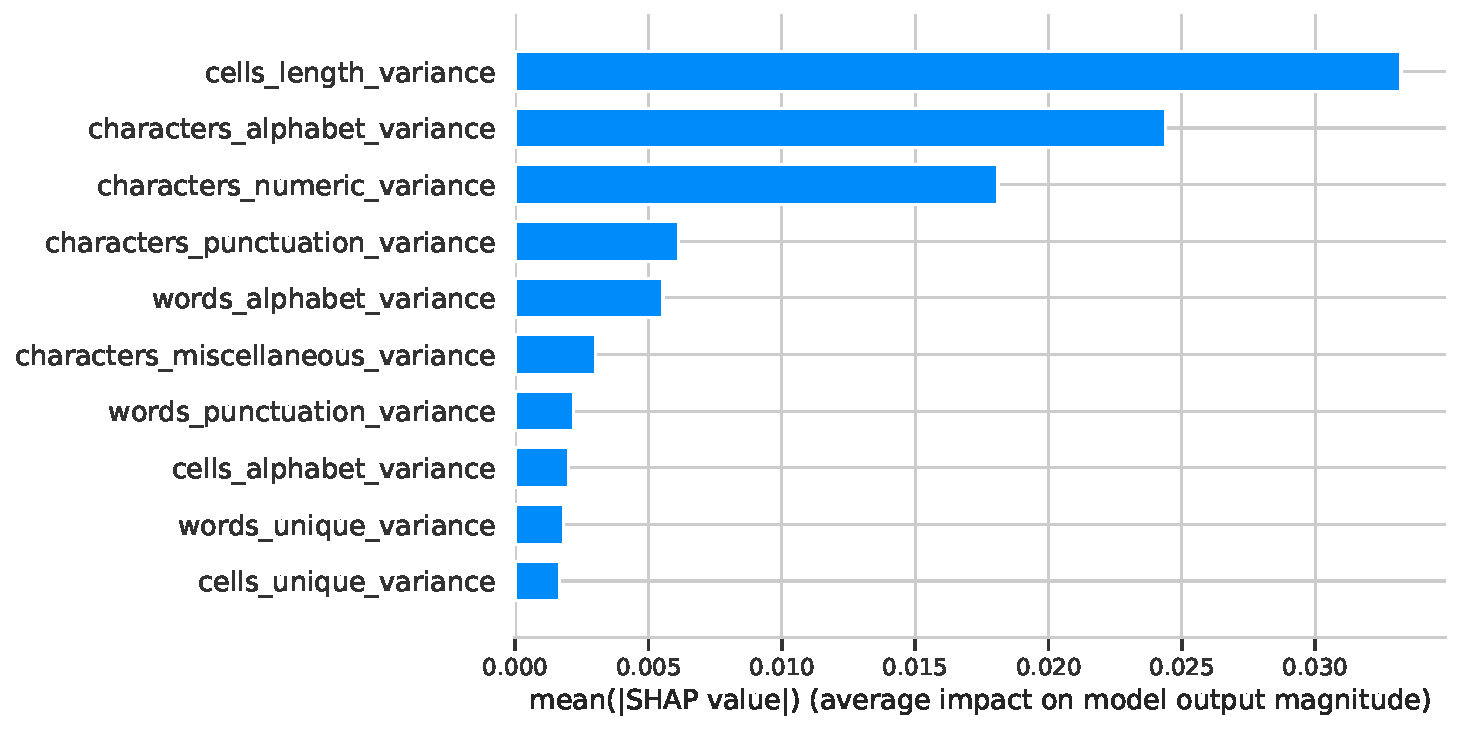
\includegraphics[width=0.9\textwidth]{thesis/Figures/RQ4/Shap_cell_f1_KATARA.pdf}
    \caption{KATARA - Top 10 influential features according to SHAP values}
    \label{fig:most_impact_features_katara}
\end{figure}

As shown in table \ref{tab:top_influence_features_KATARA}, again the most influential features for the F1 estimation are the same as for the other tools. The influences are comparable to that of ActiveClean. This can be attributed to the fact that both capture row-wise characteristics. ActiveClean tries to find common or more important words using tf-idf and KATARA tries to find common words and then map those columns of the common words to relations. 

\begin{table}[H]
\centering
\begin{tabular}{llr}
\toprule
 \# &                         Feature &         Influence \\
\midrule
 1 &         cells\_length\_variance &   -0.2 $\searrow$ \\
 2 &  characters\_alphabet\_variance &  -0.09 $\searrow$ \\
 3 &   characters\_numeric\_variance &   0.36 $\nearrow$ \\
\bottomrule
\end{tabular}
\caption{KATARA - Top 3 feature influence}
\label{tab:top_influence_features_KATARA}
\end{table}


\subsection{Raha}
For Raha, the 10 most influential features are shown in figure \ref{fig:most_impact_features_raha}. Whereas the previous tools were most impacted by the variance based features across columns, Raha is also depending slightly on other features like the maximum of punctuation words used in a column.

\begin{figure}[H]
    \centering
    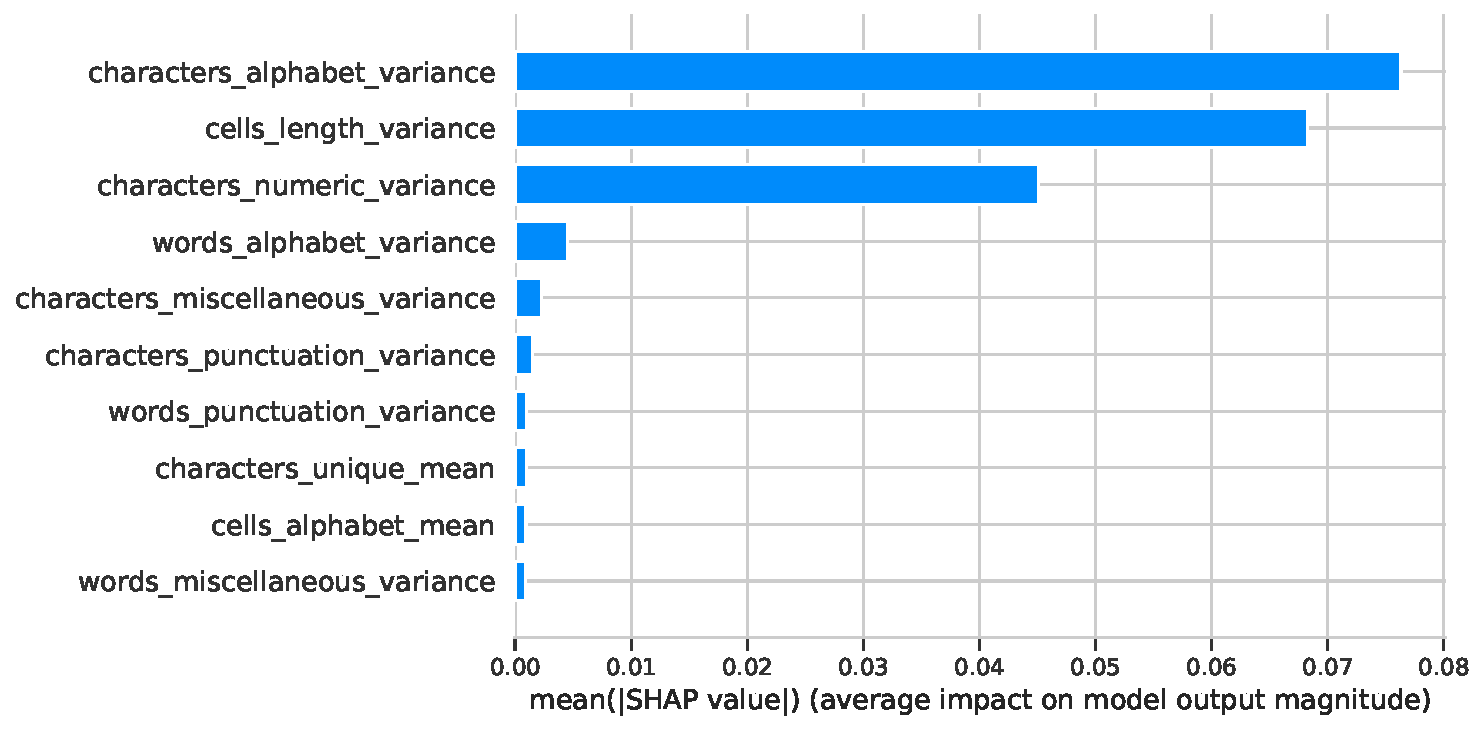
\includegraphics[width=0.9\textwidth]{thesis/Figures/RQ4/Shap_cell_f1_Raha.pdf}
    \caption{Raha - Top 10 influential features according to SHAP values}
    \label{fig:most_impact_features_raha}
\end{figure}

But, again the most influential features are characters\_alphabet\_variance, cells\_length\_variance and characters\_numeric\_variance. All have a strongly negative correlation with the performance results estimation, meaning that Raha does better when these characteristics have low variance. This means that it performs best with structured data, with same length content and without too many difference in terms of numerical characters between attributes. Because Raha is also based on the combination of underlying tools like dBoost and KATARA, it is as expected that the F1 score will be influenced by the same characteristics as these tools.

\begin{table}[H]
\centering
\begin{tabular}{llr}
\toprule
 \# &                         Feature &         Influence \\
\midrule
 1 &  characters\_alphabet\_variance &  -0.49 $\searrow$ \\
 2 &         cells\_length\_variance &  -0.42 $\searrow$ \\
 3 &   characters\_numeric\_variance &  -0.42 $\searrow$ \\
\bottomrule
\end{tabular}
\caption{Raha - Top 3 feature influence}
\label{tab:top_influence_features_raha}
\end{table}